\documentclass[conference]{IEEEtran}

%\hyphenation{op-tical net-works semi-conduc-tor}

\usepackage{syntonly}
%\syntaxonly
\usepackage{amsmath}
\usepackage{ amssymb }
\usepackage{url}
\usepackage{cite}

%------------------------------------------------------------------------------
%   list
%------------------------------------------------------------------------------
\usepackage{enumitem}
\usepackage{fancyvrb}
\usepackage{framed}
\usepackage{lipsum}
\usepackage{makecell}
\usepackage{tabu}
%------------------------------------------------------------------------------
%   algorithm
%------------------------------------------------------------------------------
\usepackage{algorithm, algorithmicx}
\usepackage[noend]{algpseudocode}

%------------------------------------------------------------------------------
%   paste code
%------------------------------------------------------------------------------
\usepackage{listings}
\lstset{showstringspaces=false}
%\lstdefinestyle{showspaces=false}
\usepackage{courier}
%\lstset{basicstyle=\footnotesize\ttfamily,breaklines=true}
%\lstset{basicstyle=\normalfont\ttfamily,breaklines=true,showspaces=false}
%\lstset{framextopmargin=50pt,frame=bottomline}
\lstset{ %
%language=python,                % choose the language of the code
basicstyle=\footnotesize\ttfamily,       % the size of the fonts that are used for the code
%numbers=left,                   % where to put the line-numbers
numberstyle=\footnotesize,      % the size of the fonts that are used for the line-numbers
stepnumber=1,                   % the step between two line-numbers. If it is 1 each line will be numbered
numbersep=5pt,                  % how far the line-numbers are from the code
backgroundcolor=\color{white},  % choose the background color. You must add \usepackage{color}
showspaces=false,               % show spaces adding particular underscores
showstringspaces=false,         % underline spaces within strings
showtabs=false,                 % show tabs within strings adding particular underscores
frame=single,           % adds a frame around the code
tabsize=2,          % sets default tabsize to 2 spaces
captionpos=b,           % sets the caption-position to bottom
breaklines=true,        % sets automatic line breaking
breakatwhitespace=false,    % sets if automatic breaks should only happen at whitespace
escapeinside={\%*}{*)}          % if you want to add a comment within your code
}

%------------------------------------------------------------------------------
%   graph
%------------------------------------------------------------------------------
\usepackage{tikz}

%------------------------------------------------------------------------------
%   url
%------------------------------------------------------------------------------
\usepackage{hyperref}

%------------------------------------------------------------------------------
%   pic
%------------------------------------------------------------------------------
\usepackage{graphicx}
\DeclareGraphicsExtensions{.pdf,.png,.jpg}
\graphicspath{{picture/}}

%------------------------------------------------------------------------------
%   title
%------------------------------------------------------------------------------
\title{Are You Coding Safely? A Guideline for Web Developers}

\author{\IEEEauthorblockN{Chun-Chan (Bill) Cheng}
\IEEEauthorblockA{Department of Computer Science and Engineering\\
Texas A\&M University\\
Email: aznchat@tamu.edu }
\and
\IEEEauthorblockN{Chia-Cheng (Jeremy) Tso}
\IEEEauthorblockA{Department of Computer Science and Engineering\\
Texas A\&M University\\
Email: jjjj222@tamu.edu}}

\begin{document}
%------------------------------------------------------------------------------
%   begin
%------------------------------------------------------------------------------
\maketitle

%\section{Introduction}
%Since the invention of the World Wide Web (WWW) by Tim Berners-Lee, it has been drastically gaining popularity in the world in the last two decades. The WWW provides a vast source of information of almost every types, ranging from stock databases to your every day weather report. Yet, in order to access the WWW, a browser is required. So came the different browsers from different cooperates and different web applications associated with different browsers we are using today. In fact, due to the proliferation of hand-holding devices in the past five years, the ubiquitous accessibility of the web browser has been a norm for today's applications. Now basically every service supports an on demand access through all kinds of devices.
%
%Web applications have many advantages over traditional ones which require installation. First of all, it works on every platform as long as there's a web browser. This takes makes developing web application a lot easier for engineers, since once a job done, it works everywhere. No more customization for different platforms. No more separated team members. Secondly, application can be patched instantly, which people usually ignore. No more asking for user to upgrade Last of all, web applications are fast deployable, fast prototype, light-weighted and is easy to get feed backs from the market.
%
%Due to these advantages, tons of frameworks and languages, from server side php to client side html, emerged for web developing. With the help of new language, new framework building an website or web application becomes very easy. Anybody can build a web application by just learning the basic of these languages. On the other hand, frameworks help you fasten the production of your web application by including third party libraries and various helpers that assist you through the development process. With the help of frameworks and new languages, no more tedious work to read through all the manual script to just understand one of the languages to write a web application.
%
%Despite the glorious future for web development, there are still many pitfall. While engineers are busy on bringing out all the functionalities, they may not have time to work on security. Which may lead to devastating consequences. Our proposal here is to provide some simple, clear but also useful guidelines to help engineer code with "good habits"
%
%Note that our goal here is not to cover every vulnerabilities, which is intuitively impossible. Our goal here is to cover as many problems as possible with minimal efforts. One might think this is not good enough. However, the concept of security is that if the value of the data in your website is less than the effort that one needs to break in, or in other words, the attacker would need to put a time that is not worth to steal your data, then, in this case, the protection should be sufficient.
%
%According to the ``Pareto principle'' , or known as the 80-20 law, most of the easy vulnerabilities should be able to eliminated, if one avoids most of vulnerability by eliminating bad coding style. It is not likely to notice every single problem without the help of scanner or static analyzer, however, by just following the guidelines of the different frameworks and languages that we propose, we believe that security breaches in the web applications may be minimized.
%
\section{Introduction}
With the proliferation of hand-holding devices,
the ubiquitous accessibility has been a norm for today's applications.
Basically every service today supports on-demand access through all kinds of devices,
and users should be able to use whatever service they like to receive.
%ranging from Macbook, iPad, to Windowns phone.
%users should be able to use Android, iOS, Windows, or Linux as they wish.
To meet this requirement, more and more service providers tend to roll
out their product as a
web application.

Web applications have many advantages over the traditional download-and-install ones:
First of all, they work on every platform as long as there's a web browser.
This takes a lot of pains off software engineers, because once a job is done, it works everywhere
-- no more customization or porting for different platforms.
%No more seperated team members.
Secondly, web applications can be patched instantly.
Every user will have the same version of application at any given time,
and it also relieves engineers from
tiresome backward-compatible requirements.
%which people usually ignore.
%No more asking for user to upgrade
%Thirdly,
Moreover,
applications can be used immediately without tedious download-install process.
This fast deployment, fast prototype, and light-weighted characteristics
greatly facilitates the project development in terms of
increasing time-to-market speed.
It also helps service providers get instant
feedback from the market, and thus altering their direction of strategy accordingly in the early stage.

Due to these advantages, lots of programming languages with their frameworks have
%, from server side php to client side html,
emerged for web development. With the help of these new tools,
building a web application is not an ``geek job'' anymore:
%becomes very easy.
anybody can build a web application by simply following some basic tutorials.
%On the other hand, frameworks help you fasten the production of your web
%application by including third party libraries and various helpers that assist
%you through the development process. With the help of frameworks and new languages,
%no more tedious work to read through all the manual script to just understand one
%of the languages to write a web application.
However, although these tools are easy to use,
%Despite the glorious future for web development,
%there are many pitfalls.
they have many pitfalls as well. For instance, in PHP 4.2.0 or lower, PHP had global variable that could be access 
any where in the application. Since PHP does not require variables to be initialized when declared, if programmers
do not take steps to protect this variable. It is likely that this variable may be compromised by malicious user by
using various of techniques, such as script injections.
%They treat

Once a developer steps on some of the vulnerability, the newly-built web application could
be another puppet controlled by malicious hackers. Continuing the example stated above, if the malicious user
decides to gain root access to the server folder of the developer's website by using the compromised variable. See the example code below:
\begin{lstlisting}[language=C]
if (authenticated_user()) {
    $authorized = true;
}

//Program continues on....

if ($authorized) {
    Sensitive_Data();
}
\end{lstlisting}
%TODO: example

Since \texttt{\$authorize} can be a global variable which was not initialized in the beginning and can be initialized even without \texttt{authenticated\_user()}. Attackers
can take advantage of this: defining \texttt{\$authorized} through various techniques, for example, defining the variable \texttt{\$authorized} through \texttt{register\_globals}. 
Boom! Your website is compromised, all the sensitive data are exposed to the attacker!

To prevent this from happening, we want to provide some simple, clear but
useful guidelines to help programmer code with ``good habits".
Normally, while engineers are busy on bringing out all the functionalities,
they do not have enough time to work on security. By following our guidelines,
they only have to pay a little extra attention, while getting a more secure application.
%the application can be more security with some
%which may lead to devastating consequences.

Note that our goal here is not to cover every vulnerabilities, which is intuitively impossible.
Our goal here is to cover as many problems as possible with minimal efforts.
You might think it's not good enough.
However, the concept of security is that if the value of the data in your website
less than the effort that one need to break in, then, in this case,
the protection should be sufficient.
%Due to its advantages, tons of framework/language emerge.
%
%with the help of new language, new framework
%building an website/web application becomes very easy.
%everybody can code
%
%And there are many more pitfall
%While engineer are busying on bring out all the functionalities,
%they may not have time to work on security.
%
%Despite the glorious future for web development, there are still many pitfall. While engineers are busy on bringing out all the functionalities, they may not have time to work on security. Which may lead to devastating consequences. Our proposal here is to provide some simple, clear but also useful guidelines to help engineer code with "good habits"
%
%Note that our goal here is not to cover every vulnerabilities, which is intuitively impossible. Our goal here is to cover as many problems as possible with minimal efforts. One might think this is not good enough. However, the concept of security is that if the value of the data in your website is less than the effort that one needs to break in, or in other words, the attacker would need to put a time that is not worth to steal your data, then, in this case, the protection should be sufficient.
%
%According to the ``Pareto principle'' , or known as the 80-20 law, most of
%the easy vulnerabilities should be able to eliminated, if one
%avoids most of vulnerability by eliminating bad coding style. It is not likely
%to notice every single problem without the help of scanner or static analyzer, however,
%by just following the guidelines of the different frameworks and languages that we
%propose, we believe that security breaches in the web applications may be minimized.

%problem statement,
%proposed technique/solution,
%a survey of related work(and comparison),
\section{Problem Statement}
Engineers have to face many pitfalls while working on an web application, such as
various framework structures and different language behaviors.
%Different servers, different languages, and different frameworks.
%such as buffer overflow, cross-site scripting, SQL injection,
On developing,
they are often too busy to pay attention on securities.
This phenomenon leads to vulnerable sites,
which could be used as a medium to carry out malicious behaviors by others.
%to resolve this issue.


%Note that our goal here is not to cover every vulneribilities, which is intuitively impossible.
%20/80 law
%most of the easy vulneribilities should be able to eliminated.
%avoid most of vulnerability by void bad coding style.
%
%It's not likely to notice every single problem without the help of scanner or static analyzer,
%however,
%
%
\section{Related Work}
Different web application vulnerability have been proposed before. In this section we will include some of the most common 
vulnerabilities that have been proposed till now. First of all, one of the most famous and most ancient attack is the sql injection 
attack which was first documented by Jeff Forristal, more know by the name of rain forest puppy \cite{Jeff}. 
 SQL injection vulnerabilities have been described as one of the most serious threats for Web applications \cite{Aucsmith} \cite{TO}. 
 In 2006, Professor Halfond classified the SQL injection attacks and proposed some countermeasures \cite{halfond06mar}.

Secondly, another famous web application attacks is the Cross Site Scripting(XSS). 
Cross-site scripting carried out on websites accounted for roughly 84\% of all security vulnerabilities documented by Symantec as of 2007\cite{symantec}. 
Cross-site scripting (XSS) attacks target an application's users by injecting code, usually a client-side script such as JavaScript, into a Web application's output. 
These attacks can cause small petty security ricks to devastating data theft depending on how sensitive are the data in the websites.

Third of all, the session management and user authentication. Web applications have to handle user authentication and establish sessions to keep track 
of each user's requests as HTTP does not provide this capability. If there is a breach in the session management of 
a web application, the attacker can then steal the user cookie and impersonate this person on the web. 
However, cookies are not accessible via non-HTTP methods, such as calls via JavaScript, by using document.cookie, and therefore cannot be stolen easily via cross-site scripting\cite{symantec}.

Last of all, the insecure direct object reference. If the web application design does not have mistake-proofing mechanism and assumes that users will always follow the application rules, 
then it is likely that a user may accidentally jump into a page that it was not granted access. This is the benign security breach, since the user may not want to steal any information. 
However, what if a malicious user starts stealing the information or to make things worse: a hacker that can read the URL or can guess the hidden field of the URL\cite{Michael}. 
If this happens, you web application can be in big trouble  \cite{Test}.

\section{Setup Local Host Website}
We will demonstrate the possible attacks if the system or any file is not configured correctly with a website we have setup. This is intended to be a raw website without any defense against any attacks. Figure 1. is the screen shot of the basic website format. All screenshot examples in the following are all attacks of this localhost website
\begin{figure}[h]
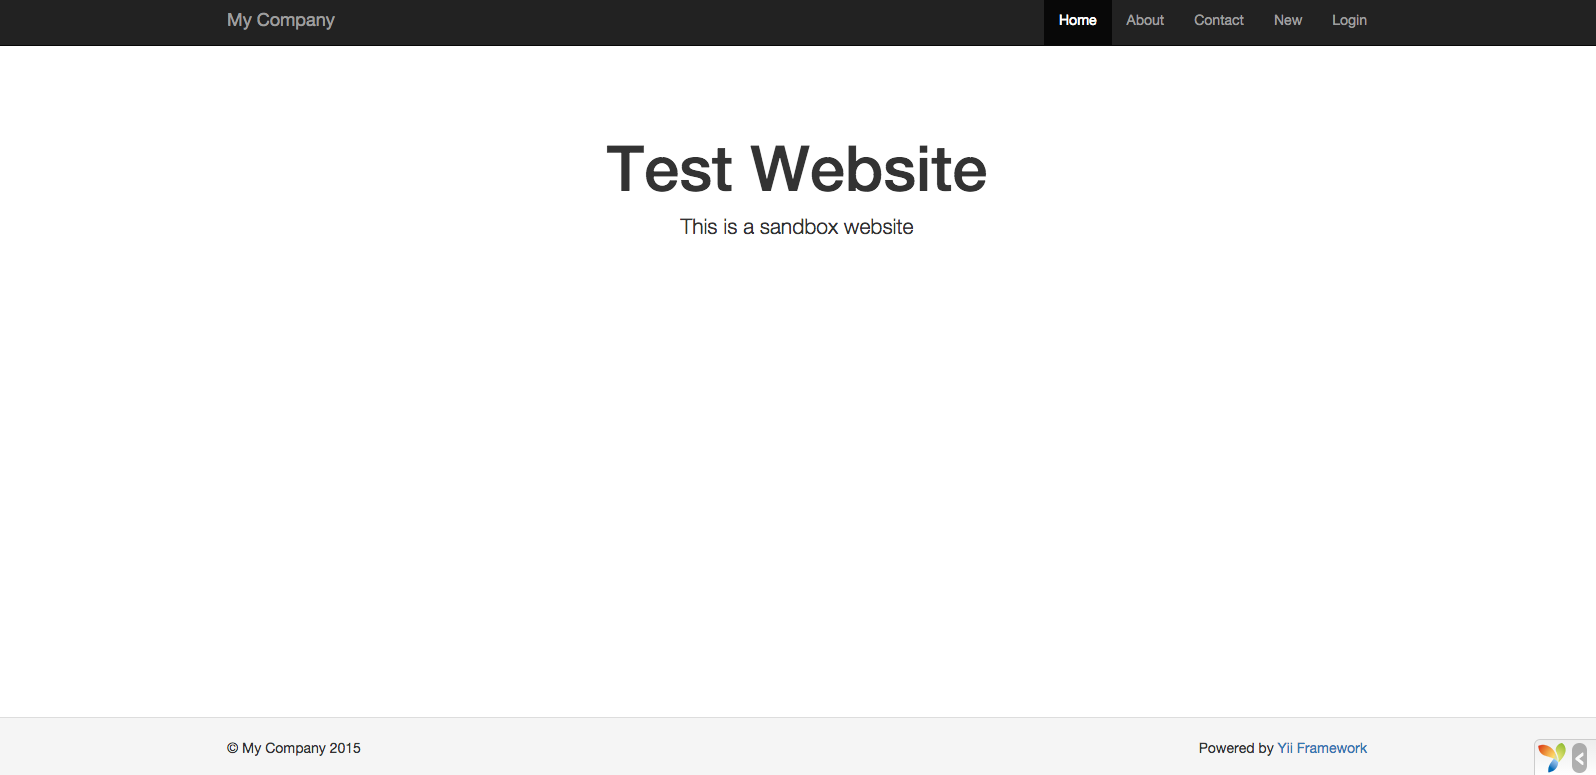
\includegraphics[width=8cm, height=4cm]{yii}
\centering
\caption{Localhost website}
\end{figure}

\section{Configuration}
In the report we will mainly focus on the things stated below
because it's the most common setup. Configuring the environment is tedious but it is crucial. In web application, there are mainly three parts to configure
which are the system (linux), the server (apache), and the language that you are writing your web application on.

\section{Apache Server Setup}
Apache server is now the most dominant http server. We can see in \cite{ApachePopularity} that till November 28 2015, Apache still had $55.7\%$ of the market share. So we will focus on the configuration for the Apache server.

\subsection{Options}
If this variable was turned on, we can see the directory of the web server. This is really not a good idea to let users see your directories. You should always check before releasing the product. Attackers could gain a lot information just by looking at this. For example, looking at this directory, attackers can now know that this is a MVC model. Attackers could easily hijack the model or controller and send the user to another malicious cite.
\begin{figure}[h]
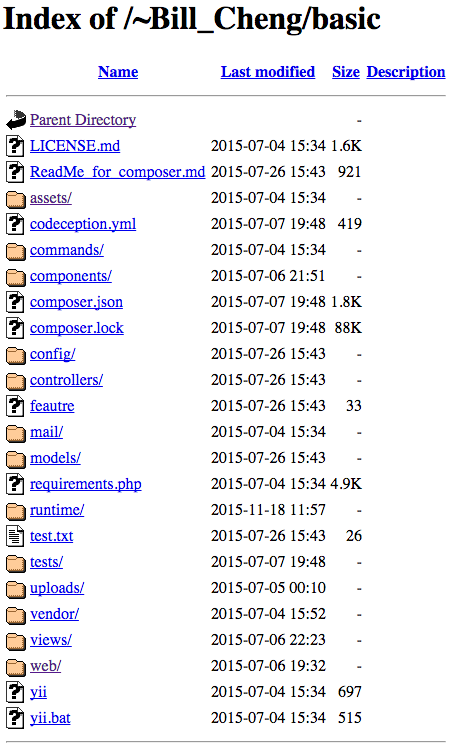
\includegraphics[width=4cm, height=6cm]{options_none}
\centering
\caption{Directory of the localhost server.}
\end{figure}

\subsection{AllowOverride}
Next, we move on to AllowOverride variable. This is an important variable because, if this is set to \texttt{'All'}, all the configuration you have configured in the APACHE file can be overridden by this file. The main purpose of having this function was because different files needed different configuration for the APACHE server, however it strongly recommended you turn this off. If attackers gain access to this file, you apache server may be in danger too.  For the example: when a user links to this server from google or facebook, it is automatically rendered to a new webpage which can be malicious. Below is the code for the malicious attack:

\lstset{escapeinside={<@}{@>}}
\begin{lstlisting}[ basicstyle=\small\ttfamily]
RewriteEngine On
RewriteCond %{HTTP_REFERER} .*google.* [OR]
RewriteCond %{HTTP_REFERER} .*facebook.* [OR]
RewriteRule ^(.*)$<@\textcolor{red}{http://malwarewebsite.com}@>
\end{lstlisting}

\subsection{ServerSignature}
This signature shows the version of APACHE and PHP, which is not an good idea because there are known vulnerabilities for out of date APACHE version which can be exploited.
\begin{figure}[h]
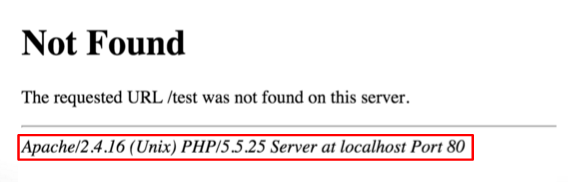
\includegraphics[scale=0.3]{serversignature}
\centering
\caption{The red box is the version number of apache and php.}
\end{figure}


\section{PHP.ini}
We will focus mainly on PHP, which covers more than $80\%$ \cite{PHPusuage} of the server side languages. We have done the initial
survey of the PHP, which includes the php.ini setup.
PHP.ini file is an important configuration file for PHP. You declare all the configuration settings in this file. Since the php.ini file is read each time PHP is initialized, it is important that
PHP developer know the basic security configuration of the PHP.ini file. Below we will give some basic guidelines for developers on what to set to the environment variable in the PHP.ini
to prevent petty attacks. Even though this configuration won't by itself fend off a determined attacker, but it will lower visibility to attacks that rely on simple techniques to scan for vulnerable targets\cite{phpini}.
 
\subsection{expose\_php}
\texttt{Expose\_php}, when turned on will tell the web server to send back the \texttt{X-Powered-By} header, in other words, \texttt{Expose\_php} will return back in every request what version of PHP is installed.

\begin{figure}[h]
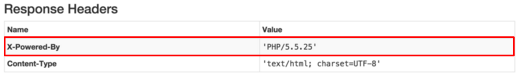
\includegraphics[scale=0.5]{exposephp}
\centering
\caption{The red box is the version number of php.}
\end{figure}


\subsubsection{Vulnerability}
If a web application is using a PHP version that is out of date or using a PHP version with known vulnerabilities, malicious attackers can exploit this vulnerability causing the web application to be 
unsecure\cite{exposephp}.

\subsubsection{Recommendation}
Setting the \texttt{expose\_php} to \texttt{off} is recommended. Even though determined attackers can still get the version of your php but it would take them more time trying to achieve this. In addition,
 the web application can stand up to simple attack scanning for specific version of php vulnerabilities. In conclusion, it is always better to set \texttt{expose\_php} to \texttt{off} than never.
 
\subsection{post\_max\_size}
The environment variable \texttt{post\_max\_size} is the variable that sets the size of \texttt{\$\_POST} which it can take.
\subsubsection{Vulnerability}
If this environment variable is not set to a realistic value, for example, if you set the value to 1024 MB, then you are giving attackers permission to put your server at stress by sending oversized POST request.\cite{postmaxsize}
\subsubsection{Recommendation}
By setting a realistic value here you can mitigate some of the damage by those attacks. This protection allows you to limit the maximum size POST request that PHP will process.

\subsection{display\_errors}
\texttt{Display\_error} is often forgotten when developers release their product. It is always not good to let user see the error. First of all, it's annoying. Second of all, it is really dangerous because there might be a logic flaw in your system which is a vulnerabilities. 
\begin{figure}[h]
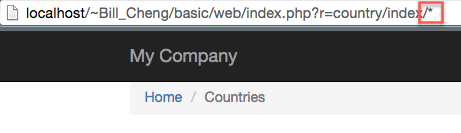
\includegraphics[scale=0.45]{displayerror}
\centering
\caption{Attackers can detect sql injection vulnerabilities by inserting ``/*" to the end of the url}
\end{figure}
For example, if a website is vulnerable to sql injection and displays error back to the users. Users will receive the following errors when \texttt{display\_errors} is turned on: \\
\begin{lstlisting}
You have an error in your SQL syntax; check the manual that corresponds to your MySQL server version for the right syntax to use near `/* ORDER BY ...'
\end{lstlisting}
\section{String I/O}
The string exploit occurs when the submitted data of an input string is evaluated as a command by the application. In this way, the attacker could execute code, read the stack, or cause a segmentation fault in the running application, causing new behaviors that could compromise the security or the stability of the system.

\subsection{Input}
We should never trust a user, and should never think that our web application is just a small project. If you are dealing with sensitive information, always keep in mind that not all user have the knowledge in security, so they might use the same password as their bank account. Therefore, when a user gives a input we should validate it and filter it. For instances, if it is a password input, we should give it a white list, only the characters in the white list is allowed. If the input is supposed to be an input of a dropdown list, checkbox, radio button, we should validate if the value is the value we intended to receive, otherwise we reject them.

\subsubsection{Server-side vs Client-side Validation}
A common mistake that developer make is only validating the user input on the client side with javascript. This can easily be bypassed when user disables javascript. Validation on the user side are beneficial but can not provide full security. In addition, the server-side validation routine will always be effective irrespective of the state of JavaScript execution on the browser. As a best practice input validation should be performed both on the client side as well as on the server side.


\subsubsection{White List}
Application whitelisting is a computer administration practice used to prevent unauthorized programs from running. The purpose is primarily to protect computers and networks from harmful applications, and, to a lesser extent, to prevent unnecessary demand for resources\cite{whitelist}. It's recommended to use whitelist when users submit a password and username.


\subsubsection{Escape}
There are two ways for developers to handle escape in user inputs. The first way is when user sends data to server, developers should escape all necessary characters in the user data and then store it into database. The second way is for developers to store data as it is and escape it when data are send to users.

There are pros and cons to these two different escaping approaches. The former one is a lot easier, escaping and then saving data to database. However, let's suppose an attacker figures out the flow in our website and manages to avoid escaping. Then the developer will have a problem of finding all data that was stored to the database unescaped.

The latter just stores data as it is but escape it once developer sends it to user. In this case, even if someone finds the flow of the  website all the developers has to do is fix the bug, since the system already assumes that data saved in database is not escaped.

Although second approach seems easier but it is a lot more prone to error. Suppose we generate HTML on server and send it to user and then decide to switch to just sending content to user via ajax, it is easy to forget that we need to escape all the data before sending it to user or implementing a new API.

To wrap things up, there are two common solutions. 1) Escape the data before storing it. 2) Store two copies of the data, one escaped, and one raw.
%pro: more general,
%con: hard to do it right
%escape function:
%1. php
%2. python

\subsection{Output}
In addition to validating all of the data the application receives, developers should also follow similar processes for the data the application will output. Some attacks such as Cross Site Scripting (XSS) can take advantage of poorly validated output to attack unsuspecting end users through the application. There are three main issues associated with output validation that developers should alway aim to keep an eye on in your application; they are data encoding, data format and data length\cite{outputvalidation}.

\subsubsection{XSS}
In a cross-site scripting (XSS) attack, the attacker injects malicious code into a web page that then runs malicious client-side script. When a user visits the infected web page, the script is downloaded to, and run from, the user's browser. This can lead to account hijacking, spread of web worms, access to browser history and clipboard contents, remotely controlling the browser, or scanning and exploiting website vulnerabilities\cite{XSS}.

\subsubsection{HTML Encoding}
A quick and straightforward way to prevent XSS is by encoding HTML responses. In fact, PHP has a library \texttt{htmlspecialchars}\cite{htmlspecialchars} that converts special characters to HTML entities. However, HTML encoding does not prevent developers from all XSS attacks. For example, suppose web server generates client side javascript , the server automatically sends html encoded scripts to the client side, in this case html encode will not stop injected script from executing.

Despite it not being able to prevent all XSS, encoding is still the correct approach, but developers would need context-sensitive encoding\cite{contextencoding}. This is when the server can recognize which context that is about to be sent to a rendering page is a unintended script or not.
%reason: avoid XSS
%method: escape?
%how to escape html?

\subsection{Conclusion}
Developers should bear in mind that not all users know about web security. So users may use the same password over multiple websites and not all website have the same security levels. If your web application becomes breached and usernames and passwords are stolen. Then the users are in immediate danger that all their other accounts may be hacked. Due to this, it is always a necessity to put most of your effort on the the string inputs and outputs.
\begin{table*}
  \centering
  \begin{tabular}{{!{\vrule width 2pt}l!{\vrule width 2pt}c|c|c|c|c|c|c!{\vrule width 2pt}}}
    \Xhline{4\arrayrulewidth}
     & Version-Based Attacks & Directory Attacks & DDOS & Flow of Program  & SQL-Injection  & Redirect Attacks & XSS\\
    \Xhline{4\arrayrulewidth}
    \textbf{Apache}: Options &  &  $\checkmark$&  &  &  & $\checkmark$ &\\
    \hline
    AllowOverride & & &  & $\checkmark$  & & $\checkmark$ & \\
    \hline
    ServerSignature & $\checkmark$  &  &  &  &  & &\\
      \Xhline{3\arrayrulewidth}
    \textbf{PHP.ini}: expose\_php & $\checkmark$  &  &  &  &  &$\checkmark$ &\\
    \hline
    post\_max\_size &  &  & $\checkmark$   &  &  & &\\
    \hline
    display\_errors &  &  &  & $\checkmark$  &  & &\\
     \Xhline{3\arrayrulewidth}
    Server Side Validation &  & $\checkmark$  &  &  & $\checkmark$  &$\checkmark$ &\\
    \hline
    Client Side Validation &  &$\checkmark$   &  &  & $\checkmark$  &$\checkmark$ &\\
    \hline
    White List &  &  &  & $\checkmark$  &  & &\\
    \hline
    Escape &  &  &  &$\checkmark$  & $\checkmark$  & & $\checkmark$\\
    \hline
    HTML-Encoding &  &  &  &  &$\checkmark$  & &$\checkmark$\\
    \Xhline{4\arrayrulewidth}

  \end{tabular}
  \caption{An Overview of the Attacks that can be prevented by the Guidelines}
\end{table*}

%------------------------------------------------------------------------------
%   Database
%------------------------------------------------------------------------------
\section{Database Access}
Almost all the information are stored in databases today,
and some of them are sensitive:
corporate IP (Intellectual Properties),
users' PII (Personally Identifiable Information),
account/password, as well as their private data.
%So many sensitive data
%and some of them are valuable.
%sensitive ones such as users' account/password,
%their private data, and their PII
These sensitive data are valuable, and thus
%Therefore,
datacases are often the key target for hackers.
Another reason why database is a popular target
is that databases are for storing information only,
so a pure information leak is all what hackers want.
With attackes such as SQL injection,
They don't even need to break into syatems to get what they want.

%There are several common issues in the deployment of databases,
%and some of them are cause by
%but not all of themFor example
To reduce potential vulnerabilities
and, if unfortunately the information in databases is leaked,
to minimize damage,
We focus on four major parts which devloper should pay attention
while working on a web application:
%at the early stage of deployment:
access control, data manipulation, storage of important data,
and backup.
Note that we use MySQL as examples here because it's one of
the most widely used LAMP \cite{LAMP} boudle.

\subsection{Access Control}
As with system and web server, database setup is also an ineluctable
step to secure web applications.
A correctly configured and updated database at the very beginning will
avoid many future problems:
not only can it better defend intrusions,
but it also can minimize or prevent errors due to incorrect design.
%TODO
%Correctly
%Setting up database correctly, as other part of the system, is a necessity.

%\subsubsection{Access Control}
The most important part for database setup is access control.
It's a universal concept that, to make system more secure,
system administor should provide users
only the least amount of privilege necessary to complete the job \cite{least_privilege}.
On one hand,
this strategy will effectively minimize the attack surface,
because one compromised account can't do much.
On the other hand, it will also force developor to follow the blueprint of
system architecture.
For exmaple, database will block the query
if a developer inadvertently write some code
that may modify the database
in a read only services.
%providing only minimal resources \cite{least_privilege}
%necessary.

In database systems,
most of the time, users only need to retrieve data, with
occasional writing, and
it's nearly impossible for users to modified the structure of database.
Therefore,
%there is no need to provide all privilege
%for every users.
our recommendation for access control is:
%Our recommendation is:
%create different users with differet privilages,
create accounts with the following differet privilages:
\begin{itemize}
\item
root
\item
database owner
\item
read-write
\item
read-only
\item
backup
\end{itemize}
What's more, there could be some
accounts specific dedicated to given tables (ex: login account with
the privilege to access only tables that store username and password)
\cite{MySQL_privilage}.
%Also, if possible, create different databases for different purpose.
%so that if a hacker gain access to one of them, others are fine.
%details are in MySQL privilage\cite{MySQL_privilage}
If the development time is truly limited, we suggest at least separate the account that
can modify the database from those that can only access it.

The following are commands to setup the privilege in MySQL:
\begin{lstlisting}[language=sql]
mysql> SHOW GRANTS FOR '[username]'@'[hostname]';

mysql> GRANT [permission] ON [database].[table] TO '[username]'@'[hostname]' IDENTIFIED BY '[password]';

mysql> REVOKE [permission] ON [database].[table] FROM '[username]'@'[hostname]';
\end{lstlisting}

And here is an example to setup an account ``username'' with read-only privilege.
You can find more details in \cite{MySQL_privilage_detail}.
%http://stackoverflow.com/questions/20036547/mysql-grant-read-only-options
\begin{lstlisting}[language=sql]
mysql> GRANT SELECT ON *.* TO 'username'@'hostname' IDENTIFIED BY 'password';

mysql> GRANT SELECT, SHOW VIEW, PROCESS, REPLICATION CLIENT ON *.* TO ...
\end{lstlisting}

%account, password, access
%information.schema?
%access permission?
%We will discuss that later.
%limited user account

%Security of the installation itself. The data files, log files, and the all the application files of your installation should be protected to ensure that they are not readable or writable by unauthorized parties.

%TODO: temporary privilage
%http://dba.stackexchange.com/questions/51500/set-password-with-a-limited-user
%an unprivileged user to modify other users, which of course is not something that can normally be done -- a user that can modify other users is, pretty much by definition, not an unprivileged user -- however -- stored procedures provided a good solution in that case, because they run with the security context of their DEFINER user, allowing anybody with EXECUTE privilege on the procedure to temporarily assume escalated privileges to allow them to do the specific things the procedure accomplishes.

Apart from access control to the information in database itself,
some databases have the privilege configuration for
the external files.
%there is also access control for database
%One of the additional tips is to
Our recommendation is to
disable local filesystem access in your SQL server if it has this feature,
because most of the time it is unnecessary, and it can be easily misused.

\subsection{Data Manipulation}
Among all the attacks, SQL injection is the most common one.
As mentioned in the previous string I/O section,
we had better take care of all the strings that read from users.
%string I/O to prvent it.
Although we can reduce most of the issues by
filtering out or escaping special characters in the strings
from external users, sometimes there are still
problems caused by internal errors,
and it's no way to block them on the border.

However, a good news is that the correct usage of database can have an
additional protections to the SQL injection issue.
The key point is to use the specialized functions provided by databases,
instead of the general ones that simply pass the content to database
without any pre-process.
For example, using proposed function can effectively
avoid some SQL injection. An exmple written in Python is demonstrated below:

%recommendation:
%use proposed function
%use proposed: avoid sql injection
%python example:
%cite: https://www.python.org/dev/peps/pep-0249/ Python Database API
%.execute ( operation [, parameters ])
%Prepare and execute a database operation (query or command).
%cur example: http://initd.org/psycopg/docs/usage.html#query-parameters
It's the incorrect way to access database:
\begin{lstlisting}[language=python]
cursor.execute("SELECT * FROM table WHERE id=%s" % (id));
\end{lstlisting}

It's the correct way to access database:
\begin{lstlisting}[language=python]
cursor.execute("SELECT * FROM table WHERE id=%s" , id);
\end{lstlisting}

These two statements look very similar, yet they are
in fact different in terms of internal operation in database.
The first one is a standard format string in python:
the placeholder ``\%s'' will be replaced by the content
of ``id'' before any operations,
and the whole query will be executed.
In other words, it's basically the same as directly
feeding the whole string in to the database,
and
apparently there is an injection problem.
%injection problem

On the other hand,
the second statement uses the proposed function.
%with paramters.
The database will pre-compute the operation before carrying out any queries,
that is, the string \lstinline[language=python]{"SELECT * FROM table WHERE id=%s"}
will be processed first before the substitution of ``\%s''.
And then the databases will apply the whole ``\%s'' directly for comparison,
instead of interpret the contain in ``\%s'' as a part of the
query control structure.
%pre-compute
Therefore,
if somebody tries to perform an SQL injection, the system will block it automatically.
This mechanics will behave as the final guard to defend problems
from both outside and inside
the application.
\begin{lstlisting}[language=python]
Warning: Truncated incorrect DOUBLE value: '1 OR 1=1'
\end{lstlisting}

\subsection{Storage of Sensitive Data}
If your systems were unfortunately intruded by hackers,
then the last thing you can do is to make them hard to get the informations
kept in database.
%And here is the benefit of encryptions.
Of course it has to be done before problems happens,
and it can be achieved by
encrypting important data.

\subsubsection{Password}
One of the most important implementation is to hide
users' passwords, and the most common practice is to hash it.
Although hashing password will still be cracked by
dictionary attacks or brute-fore attacks,
it can efficiently increase the difficulty for hackers to
get the real passwords.

Now we know the password should be hashed, to be sure, but sometimes
it requires some additional cares to do it right. The following are
some important steps for hashing passwords.

\begin{enumerate}[label=\textbf{\arabic*.}]
    \item
First of all, use cryptographic hash function. Not all the hash functions
are for secure propose, so it's important to pick up the right one.
We will discuss 
which hash functions to use in the next section.

    \item
Make sure that hashing is done on the server side,
as close the place that use it as possible.
Because
once a hash is computed, it is literally the password for the account.
Everyone with the hash value can pass the verification process. Therefore,
if the hashing is done outside the system, the hackers can just intercept the results
and use it as the key.

    \item
Add salt before hashing.
Even though hashing can provide rather strong protection for passwords,
hackers can still use many techneques to reduce the time to break it.
They can always pre-compute a table \cite{rainbow} that map
hash values to plaintexts of some strhing, and then
break the hash immediately if the value is in the table.
%while they get a
%hash value, they can simply compare it in the pre-computed table and
%get the real value.
To against this attack, the password should add some
``salt'' \cite{salt} before hashing.
The salt is just some string that append to the original value to
rearrange the plaintext to hash mapping.
It should be long enough, because the overall number of
possible value of salt means the overall number of tables that
hackers will need to pre-compute if they want to break the hash.
Any additional bit will double the table size by 2, with
negligible additional computation time in hashing, so it's
a very good trade-off.
Generally, a 32-bits or 64-bits salt would be a good option.

    \item
Use different salts for different users.
If the whole database uses the same salt, then hackers
can compute only one table for this specific salt to crack
every account, so every password should be appended with
different salt.
You might wonder then how to hide the salt,
but the truth is that the salt
doesn't have to be hidden or obscured.
Therefore, for a given account, the salt can be stored as plaintext
with other account related information.

    \item
The salt should be randomly generated and irrelevant to other
information. Because once the developor detect that the databases
are stolen, the password and the salt must be completely changed to
prevent the attack. The better practice would be generating new salt
everything the password is changed.
\end{enumerate}

The following is a php example \cite{salt_example}
for generating the hash value with a password.
%from crackstation.net \cite{salt_example}:
\begin{lstlisting}[language=php]
function create_hash($password)
{
    // format: algorithm:iterations:salt:hash
    $salt = base64_encode(mcrypt_create_iv(PBKDF2_SALT_BYTE_SIZE, MCRYPT_DEV_URANDOM));
    return PBKDF2_HASH_ALGORITHM . ":" . PBKDF2_ITERATIONS . ":" .  $salt . ":" .
        base64_encode(pbkdf2(
            PBKDF2_HASH_ALGORITHM,
            $password,
            $salt,
            PBKDF2_ITERATIONS,
            PBKDF2_HASH_BYTE_SIZE,
            true
        ));
}
\end{lstlisting}

%database been intrude,
%hash
%
%
%dictionary attacks and brute-force attacks.
%harden -> increase the time they crack
%salt
%per user -> avoid precomputed table

%recommendataion:
%such as password,
%1. hash passward
%2. add salt while hashing, rainbow table
%    don't need to hide salt
%    long enough
%django
%https://docs.djangoproject.com/en/1.8/topics/auth/passwords/
%http://stackoverflow.com/questions/749682/django-passwords Django Code

%https://en.wikipedia.org/wiki/Rainbow_table Rainbow table
%ref: https://crackstation.net/hashing-security.htm
%never tell the user if it was the username or password they got wrong. Always display a generic message like "Invalid username or password." This prevents attackers from enumerating valid usernames without knowing their passwords.



%table
%https://crackstation.net/
\subsubsection{Encryption}
Encrypting field in database is normally unnecessary,
becuase the key have to be stored somewhere in the system as well,
with the same privilege of database. And once the system is hacked,
the key will be discovered easily. Plus, it will cause additional
overhead, and make some functionality such as searching a giving pattern
very difficult to implement.
Therefore, spending your valuable time on other security issues
would be more practical.

However, if you really want to encrypt other sensitive information other than password,
there are 2
ways to do it: either encrypt it by your web application o by database itself.
Our reccommendation is to encrypt it by your web application.
Even though there is not mush difference in terms of security between
these two options, encrypting data by application has the flexibility
to change the underlining databases.
%This recommendation is not security related, it

\subsection{Backup}
In a web application, backing up the databases regularly
is crucial for avoiding any kinds of tragedies that might damage
the data, and
it is also important
from the security point of view. There are 2 issues: first,
backup can mitigate the damage caused by attacks such as CryptoLocker \cite{cryptolocker}.
It's a notorious and vicious malware that will encrypt all important files
when it infests a system, and ask for ransom.
Once files being encrypted by CryptoLocker,
there is not guarantee that you can get the key even if you pay the ransom,
so file encrypted by CryptoLocker basically could be seen as completely deleted,
and it would be a catastrophe if there is no backup.

Second, the information stored in the backup is the same as those
in the database, so its
is also a potential target for attackers.
Therefore,
both the process for backing up and the backup file should be protected as well.

The following is the flow that carry out a MySQL backup:
%ref: MySQL
%http://mirror.metrocast.net/mysql/doc/mysql-security-excerpt/5.1/en/backup-and-recovery.html
\begin{enumerate}[label=\textbf{\arabic*.}]
    \item
First, create a new user dedicated for backup. It's basically a read-only
account with some additional privilege to access system information.
\begin{lstlisting}[language=sql]
GRANT USAGE ON *.* TO 'dump'@'%' IDENTIFIED BY ...;
GRANT SELECT, LOCK TABLES ON `mysql`.* TO 'dump'@'%';
GRANT SELECT, LOCK TABLES, SHOW VIEW, EVENT, TRIGGER ON `myschema`.* TO 'dump'@'\%';
\end{lstlisting}

\item
Create \lstinline{.my.cnf} in home directory to enable auto-login
without expose the account and passward. Note that the file should be
created by root.
%Write the script as root, put the password into root's .my.cnf (with permissions 600). You can then run mysql commands without ever having to pass the password.

\begin{lstlisting}
cat ~/.my.cnf
[mysqldump]
user="username"
password="password"
shell> chmod 600 .my.cnf
\end{lstlisting}
%%shell> mysql --defaults-file=/home/francis/mysql-opts

\item
Write a script as root, and put all the commands for backup in it.
If you want to use logical backup, use \lstinline{mysqldump}.
\begin{lstlisting}
mysqldump --all-databases > backup.sql
\end{lstlisting}
%simple steps:
%mysqldump (logical backup)

\item
Remember to add commands that encrypt the backup file.
%entrpyted
%-> encrypting archives to mitigate the insider-risk.
%
\begin{lstlisting}
openssl aes-256-cbc -in plan-text.txt -out message.enc
openssl aes-256-cbc -d -in message.enc -out plain-text.txt
\end{lstlisting}

\item
Use crontab or other system daemon to automatically execute you backup script.
The numbers and stars below stand for min, hour, day, month, and weekday.
%cron %how to use cron
\begin{lstlisting}
crontab -e
01 01 * * * /path/to/your_script
\end{lstlisting}
%minute (0-59), hour (0-23, 0 = midnight), day (1-31), month (1-12), weekday (0-6, 0 = Sunday), command

\end{enumerate}




%but entryped
%backup
%-> crypolocker




%Databases also contain a networking interface, and so hackers are able to capture this type of traffic to exploit it. To avoid such a pitfall, administrators should use SSL- or TLS-encrypted communication platforms.


%------------------------------------------------------------------------------
%   crypto
%------------------------------------------------------------------------------
\section{Cryptographic Utilities}
%Needless to say, the
%network
Everybody knows that it's important to encrypt data while sending them over the internet,
yet not everybody does it right.
As the technologies of cryptography evolving,
they become more and more complicated.
%It's not the simple one-key-one-algorithm anymore.
Normally, in an encrpyted communication, there are more the 1 keys involved,
along with parameters, nonces, and different kinds of operation modes;
some of them should be kept secret, while others are not;
some of them can be reuse, while others must change every time.
%some are public, some should be kept secret,
%set up, %nonce, %some
It's overwhelming for most of developors, and even an expertise might sometimes get it wrong.

%key, function, implementatino, nonce.
One of the exmples is the famous Sony PlayStation 3 issue \cite{PS3_Jailbreak}:
Sony used ECDSA \cite{ECDSA} but didn't change the ephemeral key, so the
private was calculated easily.
%cite https://en.wikipedia.org/wiki/PlayStation_Jailbreak
%cite https://en.wikipedia.org/wiki/Elliptic_Curve_Digital_Signature_Algorithm
Other well-known example is the
side channel attack such as differential power analysis \cite{differential}:
%cite https://en.wikipedia.org/wiki/Side-channel_attack
The implementation is correctly, but functional correctness is not sufficient to
be crpytographically secure.
%For the
%lack of knowledge
%looks fine but indeed not

%cite http://www.nist.gov/ NIST
%cite https://www.owasp.org/index.php/Guide_to_Cryptography OWASP guide
%cite http://csrc.nist.gov/groups/ST/toolkit/documents/dss/NISTReCur.pdf NIST ecc recommendation
%\subsection{general concept}
%To support developors, we concluded the following guildlines:
Our recommendations for applying cryptographic functions are as follows:
%Three most important concepts
\begin{enumerate}[label=\textbf{\arabic*.}]
    \item
Always encrypt your communication. You never know what information would help hackers
break into your syatem, even if they appear to be harmless. Like the side-channel
attack mentioned above, every small difference of data could be a hint of
how your system works and what's in it, and it finally leads to
true vulnerability. Therefore, since the modern computer, even cellphone,
is faster enough to perform symmatric encryption, just take adventage of it.

    \item
Use well-known standards, don't invent the encrpytion algorithm yourself.
The seemly unbreakable Enigma \cite{enigma} in World War II was still cracked by
the technology at that moment; not to mention plenty of techniques,
such as differential cryptanalysis \cite{diff_crypto},
have invented since then. Without thorough analysis, nobody knows
whether a encryption scheme or algorithm
have any defect in it. Even if the detail of the algorithm might
keep as a secret to defend attacks for a given time,
eventually it will be known by attacker.
Modern encryption algorithms, such as AES, 3DES, have been well-studied and proven to be
very secure, and most of them have standard documents and convenient libraries,
so there is no reason to invent a new one.

%TODO: NIST \cite{NIST}
%TODO: NXP mifare \cite{mifare_break}
    \item
%use the good one
Use the up-to-date standard. Even though most of the common algorithms look
fine, and are still widely adopted.
Some algorithms such as md5 have been proved to be unsafe \cite{md5_break}.
Old system might have some compability issues to use the new standard;
however, if you are developing a new web application, there is no reason
not to use the latest one.

\begin{table}[H]
    \centering
    \begin{tabular}{ l | l | l}
            Type  & recommendation & out-of-date\\\hline
            Symmatric  & AES-128 & 3-DES\\
            Assymatric & RSA-2048 & RSA-1024\\
            Hash       & SHA-256 & md5\\
            Signature & ECDSA-256 & RSA-1024\\
            Stream  & AES-CTR-128 & RC4
    \end{tabular}
    \caption{Cryptographic algorithms to use}
\end{table}


    \item
Use libraries, don't implement algorithm yourself.
Again, even if an algorithm is proven to be secure, an
invalid implementation might still undermine it.
Some simple functions
are totally different if it's implemented to in the sense of security.
For eaxmple, a normal string compare function will
compare 2 strings from the first character:
if it encounter any different charater, it will return the
result that these 2 strings are different.
But when it comes to security, this algorithm is highly unsecure.
because the attacker can use the differece of computation time
to get the information about how many characters are the same
at the beginning of the 2 strings, which will lead to the break
of the whole system.
%(even  RNG)

    \item
Use it right. Most of the algorithms are complicated, so make sure to
follow guides carefully for setup. 
Documents such as those published by NIST \cite{NIST} is a very good source.
\end{enumerate}

%We will provide a more completet list of recommended functions,
%for hash, symmetric and assymetric encropyion,
%in many common web-debelop languages
%in the final report.

%\subsection{asymmetric}
%\subsection{symmetric}
%\subsection{hash}
%\subsection{RNG}
%\subsection{SHA, AES, RSA, ECC?}
%provide some python function
%%cite: https://docs.python.org/2/library/hashlib.html#module-hashlib Python hashlib
%
%%cite: https://en.wikipedia.org/wiki/Cryptographic_hash_function#Cryptographic_hash_algorithms
%Don't use MD5, SHA-1
%Use SHA-2
%%cite: https://en.wikipedia.org/wiki/SHA-2
%
%good function for
%1. hash
%2. encrpytion
%3. randeon number geneerator
%%https://pypi.python.org/pypi/pycrypto
%python crypto function
%
%key strength match
%because the weakest part
%
%\subsection{SSL}
%library and their setup?


%------------------------------------------------------------------------------
%   
%------------------------------------------------------------------------------
\section{Useful Tools}
It's undoubtedly that we need plenty of tool to help us
develop our web application. Aside from editor, debugger,
linter, etc. Some tools can help us enhance the secuirty of our application.
%Many tools such as packer or fuzzer can help developers
%further improve the quality of web application.
%We will introduce some tools after doing some experiments on them.
%use tool to help us
%\subsection{PaaS}
%Aamazon AWS?

\subsection{Packer (Minifier)}
Packer or minifier can rearrange your code without change its
functionality.
For script language, especially Javascript, it is a very useful tool.
Using packer before releasing your code have 2 fold advantages:
First of all, it can remove all the comments, white space, newline, etc.,
as well as
shorten function and
variable names.
Since script language is executed by interpreter on-the-fly, this reduction
will speed up the execution.
Second, it can obfuscate code and make it hard to be reverse engineered.

%1. harden code
%2. enhance runtime

\subsection{Fuzzer and Scanner}
Everybody will make mistakes, and it is good to have other's check for you.
For web applications, run some fuzzer or scanner to hit potential problems
is a good option.
They can rule out some stupid bugs, which are highly possible
to be discovered as well by attackers by running similar tools.
%penetration test.
%1. test

%\section{TDOO}
%1. build case to test
%2. detail usage
%3. test whether the guildlines are truly useful
\section{Conclusion}
In this paper, we categorized several essential points- Backend: Apache Server setup, Database Access PHP.ini setup, Front-end: String I/O, Cryptography, and last of all some useful tools
for future developers to follow. 

It is our notion that by following the rules we proposed, majority of the bugs or malicious attacks can be
prevented. We set up a local host website to test the guidelines and ran automated script attacks on the website to see the security breaches. Most attacks were prevented
if our guidelines were followed. However, it should be noted that more sophisticated attacks may need further security implementation since our guidelines are the basic requirements
for web developers especially for fresh web developers.

In conclusion, our target here is to provide some simple, clear but useful guidelines
to help engineer code with "good habits", and thus
eliminating most of vulnerabilities with minimal efforts.
\bibliographystyle{unsrt}
\bibliography{references}
%------------------------------------------------------------------------------
%   end
%------------------------------------------------------------------------------
\end{document}


